\documentclass{beamer}
\usetheme{Darmstadt}
\usepackage{graphicx, caption, listings, xcolor}
\usepackage[T1]{fontenc} %Stops attempting to use speech marks in code listings.
\usepackage[style=authortitle-ibid,backend=biber]{biblatex}
\addbibresource{refs.bib}
\graphicspath{ {images/} }

\lstset{
    columns=fullflexible,
    basicstyle=\ttfamily,
    frame=single,
    breaklines=true,
}

\title{Pothole Reconnaissance Network}
\subtitle{Tech for Good}
\author[Smith, Tsaris, Turnbull, Waldock]{H.~Smith \and A.~Tsaris \and L.~Turnbull \and L.~Waldock}
\institute[5J]{Group 5J}
\date{\today}

\AtBeginSection[]
{
  \begin{frame}
    \frametitle{Table of Contents}
    \tableofcontents[currentsection]
  \end{frame}
}

\begin{document}


\frame{\titlepage}

\section{The Problem}

\begin{frame}{What is a pothole?}

\begin{columns}

\column{0.6\linewidth}

How potholes develop:
\begin{enumerate}
    \item Cracks in the road develop from wear-and-tear by vehicles.
    \item Water seeps into these cracks.
    \item The water freezes, expanding the cracks --- the pothole is formed.\footnote[frame]{\cite{how-are-potholes-formed}}
\end{enumerate}
Potholes in the road are a challenge and a danger to many drivers and cyclists.

\column{0.4\linewidth}
\begin{figure}
    \includegraphics[width=3.5cm]{potholes.jpg}
    \caption{Picture of a pothole\footnote[frame]{\cite{pothole-pic}}}
\end{figure}

\end{columns}

\end{frame}

\begin{frame}{Financial Risks}

    They pose a \alert{financial} risk due to the cost of vehicle repair.

    \begin{itemize}
        \item Cars are often damaged after driving over potholes.
        \begin{itemize}
            \item cracks on windscreen
            \item burst tyres
            \item damage to suspension
            \item and more…
        \end{itemize}
        \item Drivers called out the RAC to 5,153 breakdowns caused by potholes in Q4 2023 \footcite{car-breakdowns}.
    \end{itemize}
\end{frame}

\begin{frame}{Health Risks}

They also pose a risk to \alert{health} as:

    \begin{itemize}
        \item Cars can lose control after driving into them, potentially crashing into other cars, cyclists and pedestrians.
        \item Drivers may attempt to swerve around them when it is unsafe to do so.
        \begin{description}
            \item[e.g.] driving close to parked cars, abruptly driving into another lane, etc.
        \end{description}
        \item Cyclists can crash into them, potentially flipping-over and injuring themselves.
    \end{itemize}

    \begin{alertblock}{Intertwined Problems}
        All health risks can become financial risks!

        From private healthcare costs to lost wages.
    \end{alertblock}

\end{frame}

\begin{frame}{Why Solve This Issue?}
    \begin{itemize}
        \item Until we use indestructible road material, potholes will always be an issue --- and so will these risks.
        \item However, we can take steps to \emph{mitigate} this by filling potholes as often and promptly as possible.
        \item A complimentary system can be created to alert local councils of the location of potholes, so that they can be repaired swiftly.
    \end{itemize}

    \begin{block}{From the BSC Code of Conduct:}
    ``[You shall] have due regard for public health, privacy, security and wellbeing of others and
    the environment''\footnote[frame]{\cite{bcs-coc}}
    \end{block}
\end{frame}

\section{The Current Solution}

\begin{frame}{Reporting a Pothole}
    Potholes can currently be reported online through government websites.
\end{frame}

\begin{frame}
    Users can access \url{https://www.gov.uk/report-pothole}, and enter the postcode for the pothole found.
    \begin{figure}
        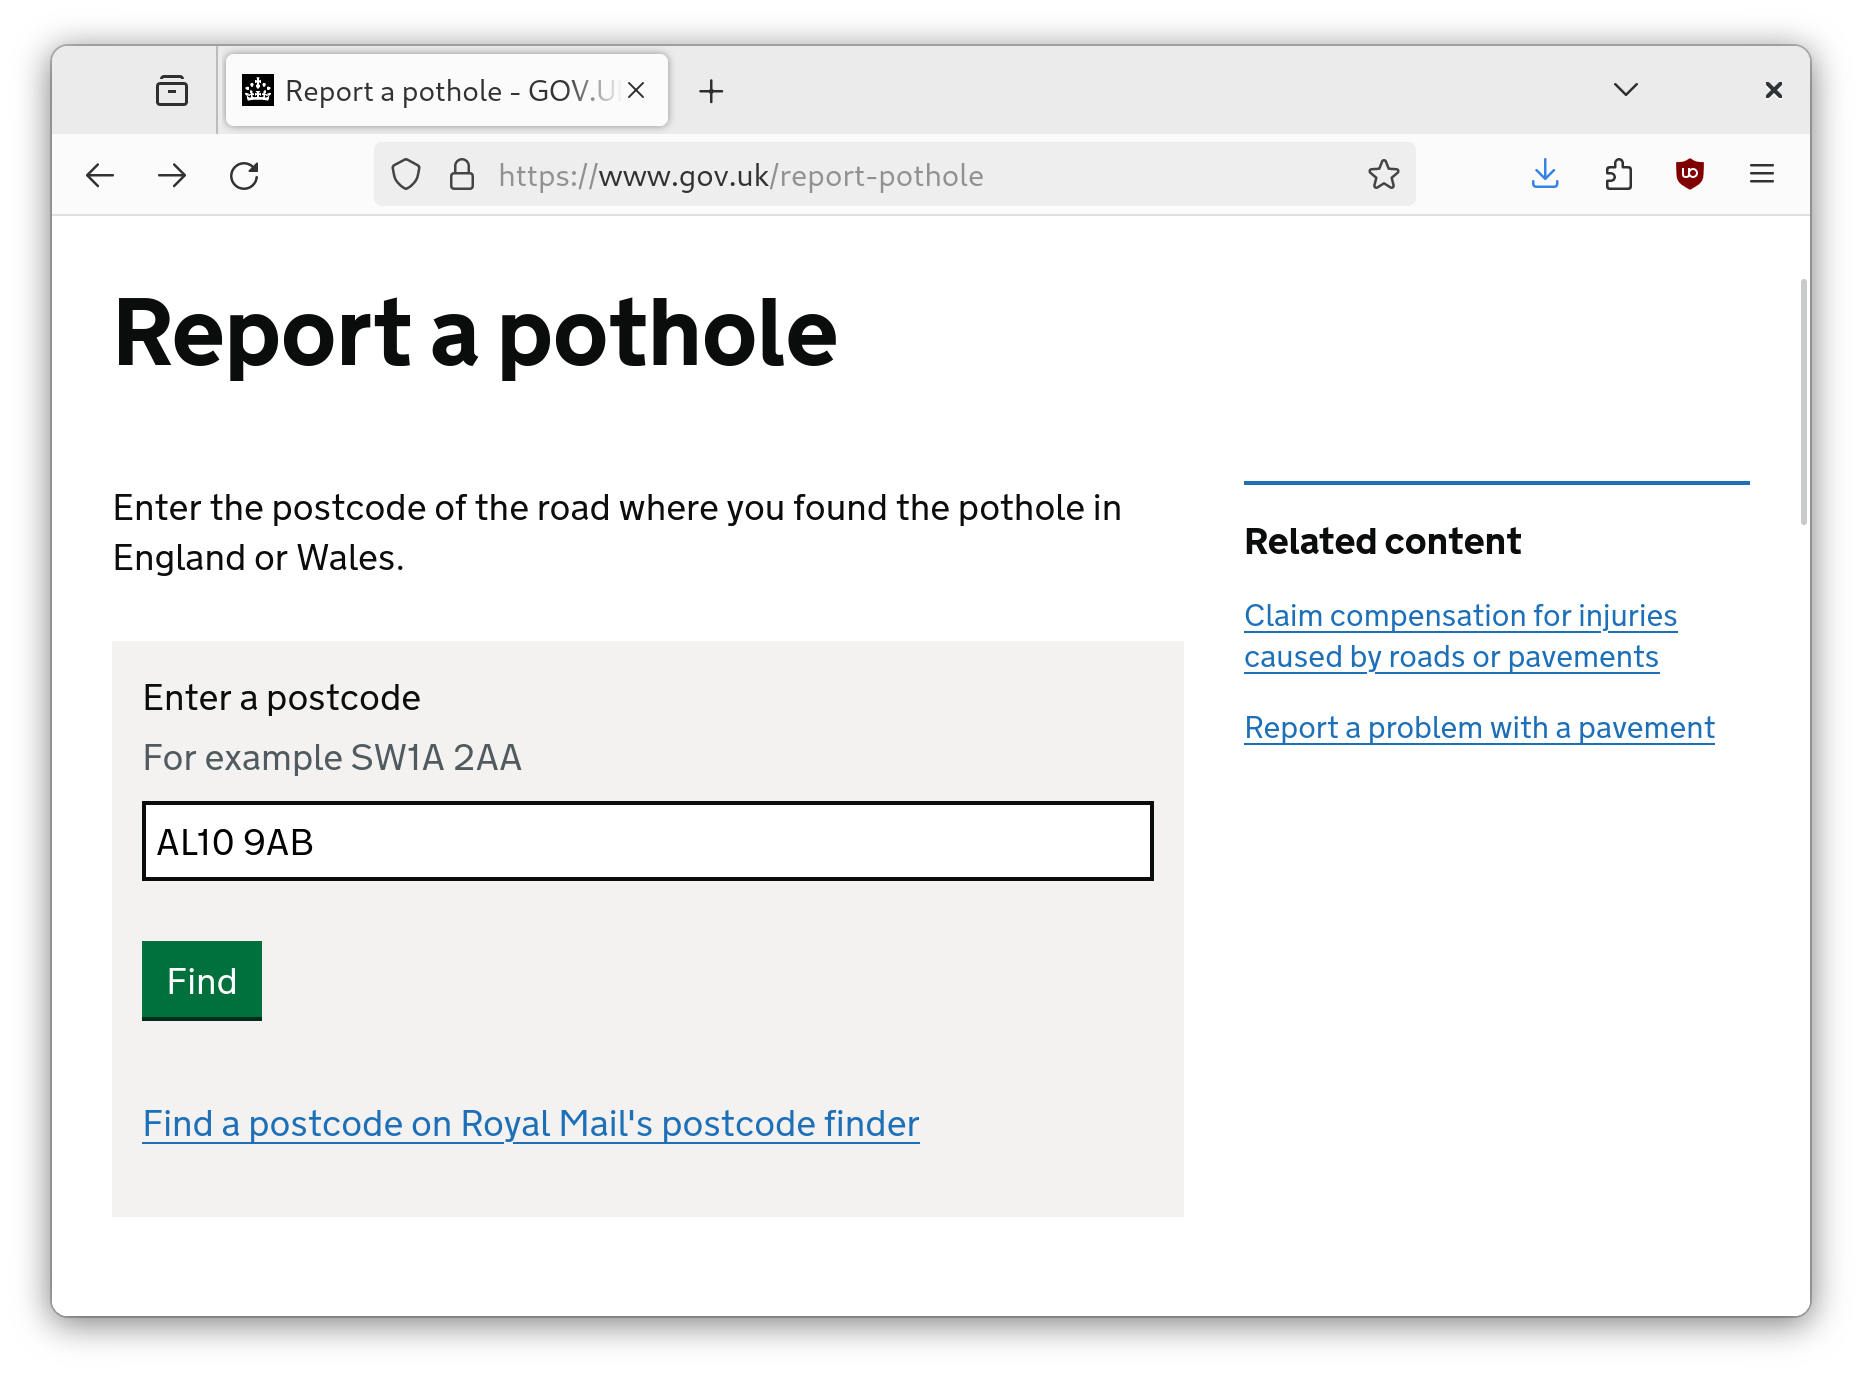
\includegraphics[width=8.3cm]{gov-uk.png}
        \caption{A screenshot of GOV.UK's site to report a pothole}
    \end{figure}
\end{frame}

\begin{frame}
    They are then redirected to their local council's site.
    \begin{figure}
        \includegraphics[width=8.3cm]{hertfordshire-report.png}
        \caption{A screenshot of Hertfordshire County Council's page to report a pothole}
    \end{figure}
\end{frame}

\begin{frame}{Problems With This}
    Motorists cannot report potholes in real time.
    \begin{itemize}
        \item It would be unsafe and illegal to use these websites while driving \footcite{highway-code}.
        \item Therefore, users must wait until they safely park before they can submit a report.
    \end{itemize}
\end{frame}

\begin{frame}{Problems With This}
    By the time users can safely access the website(s):
    \begin{itemize}
        \item They may have forgotten about the pothole, and likely won't report it.
        \item Or they may remember the pothole, but cannot recall its exact location (needed in the report).
        \item Or they may not simply have the time or patience to manually submit a report for every pothole they find on the road.
    \end{itemize}
\end{frame}

\section{Our Solution}

\begin{frame}{Automated Reporting}
    There will be two `clients' of the system --- the road users, and the local councils.

    \begin{itemize}
        \item Compatible vehicles will be programmed to automatically generate a report when a shock on the suspension is detected with force above a certain threshold.
        \item The car's computer will be the control system for this.
        \item Locations with potholes are likely to trigger this shock-detection far more than smooth parts of the road.
        \item This report includes the current geolocation and shock strength and is sent to the local council.
    \end{itemize}
\end{frame}

\begin{frame}{The Council's Side}
    \begin{itemize}
        \item The local council can then receive this location data, and use it to visualize where these `pain points' (i.e., potential potholes) are on a map.
        \item Locations with numerous reports are likely pothole locations --- locations with only one or two reports are likely false positives and won't be shown.
        \item Potholes with higher reported shock strengths are marked as high-priority, as they are more dangerous.
        \item The location data can be filtered by priority level and road type to better facilitate planning of repairs.
        \item Each council can only see data relevant to their own geographic area.
    \end{itemize}    
\end{frame}

\begin{frame}
    \begin{figure}
        \includegraphics[width=10.8cm]{map.jpg}
        \caption{Mock up of the council-side pothole report map}
    \end{figure}    
\end{frame}

\begin{frame}{Use of Car Cameras}
    \begin{columns}
        \column{0.6\linewidth}

        \begin{itemize}
            \item Many newer cars have in-built cameras for security and driver ease of use.
            \item The front camera --- paired with image recognition --- can be used to scan for potholes in the road.
            \item A report will be generated and sent when a pothole is detected.
            \item The front camera can also detect when something is \alert{not} a pothole (more on this shortly).
        \end{itemize}

        \column{0.4\linewidth}

        \begin{figure}
            \includegraphics[width=4.3cm]{front-car-camera.jpg}
            \caption{Picture of a car's front camera in operation\footnote[frame]{\cite{front-camera-picture}}}
        \end{figure}
    \end{columns}
\end{frame}

\begin{frame}{Why Both?}
    Why have two systems to detect potholes?

    Isn't this redundant?
\end{frame}

\begin{frame}
    \begin{columns}
        \column{0.55\linewidth}

        \begin{block}{Advantages of suspension system}
            \begin{itemize}
                \item Can detect potholes visually obscured by snow, puddles, and fords.
                \item Less prone to error, due to the simpler implementation --- does not rely on `experimental' AI.
                \item Can be used in a broader variety of cars (ones that don't have front-facing cameras).
                \item Pothole danger can be ranked based on severity of impact.
            \end{itemize}
        \end{block}

        \column{0.45\linewidth}

        \begin{block}{Advantages of front camera}
            \begin{itemize}
                \item Can detect potholes even if the car drives over or around them.
                \item Should (in theory) \alert{only} detect potholes, rather than anything that causes a bump.
            \end{itemize}
        \end{block}

    \end{columns}

    \vspace{0.4cm}
    Using \emph{both} systems allows either system to overcome the limitations of the other!
\end{frame}

\begin{frame}{Filtering}
    We want data sent to local councils to be as accurate as possible.
    \begin{itemize}
        \item If both the suspension sensors and camera are active, feedback from the camera can reduce false-positives from the suspension sensors.
        \item It does this by identifying objects that will likely cause a `bump' that are \alert{not} potholes.
        \begin{description}
            \item[i.e.] speed bumps, the curb, debris, etc.
        \end{description}
        \item The control system can then take this as information that the upcoming shock of the suspension can be ignored.
        \item \alert{No} report is sent in this case.
    \end{itemize}
\end{frame}

\begin{frame}{Server-Side Filtering}
    A control layer at the server's side can further reduce false-positives by comparing suspected pothole location data with locations of known obstacles like speed bumps.

    \begin{itemize}
        \item Locations of speed bumps that match locations of suspected potholes can be removed automatically.
        \item Useful for:
        \begin{itemize}
            \item Reports from cars that have suspension sensors but no front camera.
            \item When the front camera fails to recognize a speed bump.
        \end{itemize}
        \item Downside to \alert{only} using this is that it won't filter out dynamic suspension triggers like hitting the curb or crashes.
    \end{itemize}
    
    \begin{exampleblock}{Example in Python}
        Assuming each variable is a \lstinline|set| of location data:

        \lstinline[language=Python]|potholes = reports - speed_bumps|
    \end{exampleblock}
\end{frame}

\begin{frame}{Sat-Nav Integrations}    
    \begin{itemize}
        \item The system will integrate with sat-nav systems to warn drivers and cyclists of potholes.
        \begin{description}
            \item[i.e.,] Google Maps and Apple Maps 
        \end{description}
        \item This prepares the user to slow down in good time.
        \item In addition to visual prompts, warnings will be communicated through audio prompts.
        \item This informs the user without them being distracted or taking their eyes off the road.
        \item Integrating with existing sat-nav systems --- instead of creating a new one --- means that views are not forced on the user (requiring the use of a new sat-nav system for this functionality), empowering user choice as per Beard \& Longstaff's ethical guidelines \footcite{principles-for-good-tech}.
    \end{itemize}
\end{frame}

\begin{frame}{Sat-Nav Integrations}
    \begin{columns}
        \column{0.4\linewidth}
        \begin{figure}
            \caption{TODO: Add screenshot of warning}
        \end{figure}

        \column{0.6\linewidth}

        \begin{exampleblock}{Audio prompt example}
            ``Caution! Pothole in 30 yards.''
        \end{exampleblock}
    \end{columns}
\end{frame}

\begin{frame}{Pothole Repairs}
    \begin{columns}
        \column{0.5\linewidth}

        \begin{figure}
            \includegraphics[width=4.2cm]{mark-as-filled.jpg}
            \caption{Mock-up of council-side UI}
        \end{figure}

        \column{0.5\linewidth}

        \begin{itemize}
            \item As repair contractors fill potholes in the road, they or the council can mark them as filled.
            \item This will remove reports of the pothole --- up until the time of its repair --- from the system.
            \item This also removes warnings of the pothole from users' sat-nav systems.
        \end{itemize}
    \end{columns}
\end{frame}

\section{Ethical Concerns}

\begin{frame}{Economic Bias}
Requiring the use of vehicles with these modern features may introduce economic bias, as these vehicles are often more expensive.

\begin{itemize}
    \item This means poorer areas could have few data about potholes, as inhabitants won't likely have the means to generate a report with this system.
    \item In turn, this could lead to the council overlooking these particular roads when organizing repairs.
    \item This makes roads in poorer areas more dangerous.
\end{itemize}
\end{frame}

\begin{frame}{Combatting Economic Bias}
    We could implement a system that lets users make manual (hands free) reports via the sat-nav system while driving.

    \begin{exampleblock}{Example phrase to submit a report}
        ``Hey Google, report a pothole here.''
    \end{exampleblock}

    However, this could be problematic for a number of reasons.
\end{frame}

\begin{frame}{Bad Actors}

    TODO mention consideration of bad uses.
\end{frame}

\begin{frame}{Distracting Users}
    The original implementation of the system is designed to be \emph{invisible} to the user.
    Manual reporting may go against Balkan \& Kalbags's Ethical Heirarchy of Needs \footcite{ethical-hierarchy-of-needs}.

    \begin{itemize}
        \item Currently, potholes are reported automatically without user-input.
        \item Introducing manual reporting would undo   
        \item Manual reporting may go against Balkan \& Kalbags's Ethical Heirarchy of Needs \footcite{ethical-hierarchy-of-needs}.
        \item A manual report may divide the user's attention from the road.
        \item This opposes the 
    \end{itemize}

    TODO mention wasting the user's time.
\end{frame}

\section{Conclusion}

\begin{frame}{The End}
    Thank you for listening.
    
    Any thoughts or questions?
\end{frame}

\begin{frame}[allowframebreaks]{References}
    \printbibliography
\end{frame}

\end{document}